\begin{tikzpicture}[transform canvas={scale=0.9}] 
  \begin{scope}[yshift=0.2\textwidth]
    \begin{scope}[xshift=0cm]
      \node [mybox] (all) at (0, 0) {
        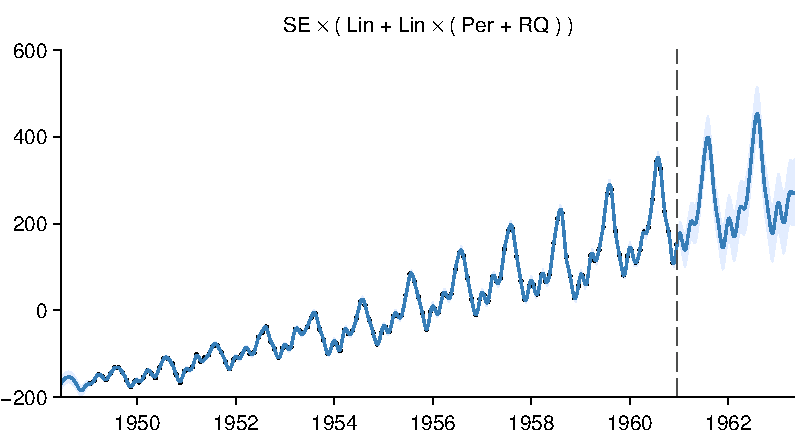
\includegraphics[trim=0 0 0 1.2cm, clip, width=0.8\textwidth, height=0.3\textwidth]{figures/01-airline-months_all.pdf}
      };
    \end{scope}
  \end{scope}
  \begin{scope}[yshift=0\textwidth]
    \begin{scope}[xshift=0cm]
    \end{scope}
  \end{scope}
  \begin{scope}[yshift=0.3\textwidth]
    \begin{scope}[xshift=4.12cm]
        \node [mybox, below of=all] (equals) at (0, 0) {\Huge{$=$}};
    \end{scope}
  \end{scope}
  \begin{scope}[yshift=-0.1\textwidth]
    \begin{scope}[xshift=-0.3\textwidth]
      \node [mybox] (all) at (0, 0) {
        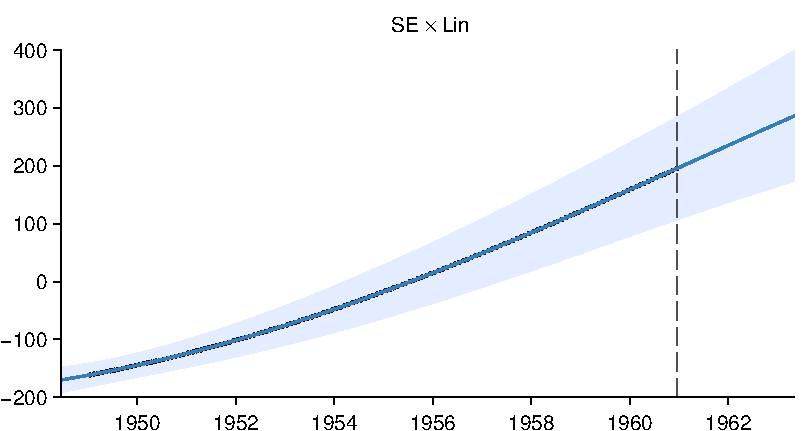
\includegraphics[trim=0 0 0 1.1cm, clip, width=0.5\textwidth]{figures/01-airline-months_1.pdf}
      };
    \end{scope}
    \begin{scope}[xshift=+0.3\textwidth]
      \node [mybox] (all) at (0, 0) {
        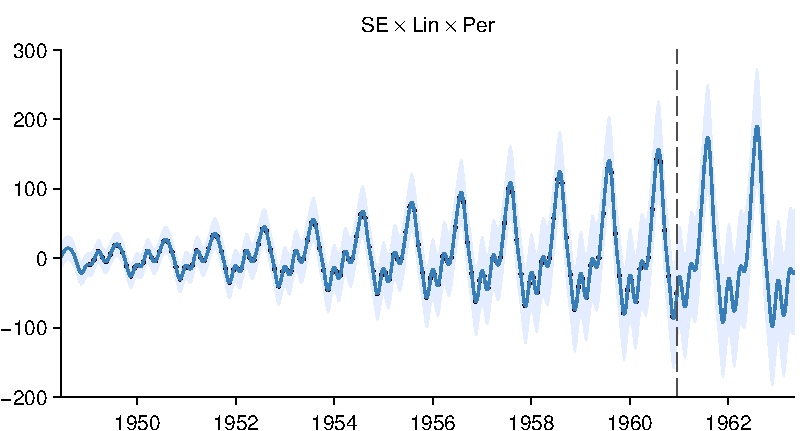
\includegraphics[trim=0 0 0 1.1cm, clip, width=0.5\textwidth]{figures/01-airline-months_2.pdf}
      };
    \end{scope}
  \end{scope}
  \begin{scope}[yshift=-0.15\textwidth]
    \begin{scope}[xshift=0cm]
        \node [mybox, below of=all] (equals) at (0, 0) {\Huge{+}};
    \end{scope}
  \end{scope}
  \begin{scope}[yshift=-0.35\textwidth]
    \begin{scope}[xshift=-0.3\textwidth]
      \node [mybox] (all) at (0, 0) {
        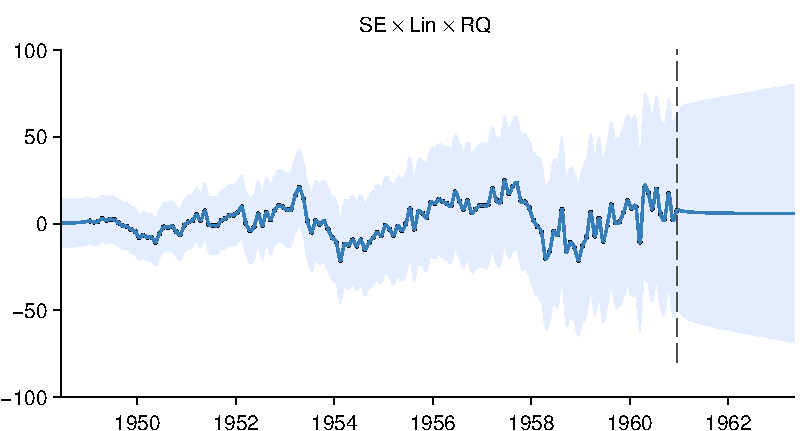
\includegraphics[trim=0 0 0 1.1cm, clip, width=0.5\textwidth]{figures/01-airline-months_3.pdf}
      };
    \end{scope}
    \begin{scope}[xshift=+0.3\textwidth]
      \node [mybox] (all) at (0, 0) {
        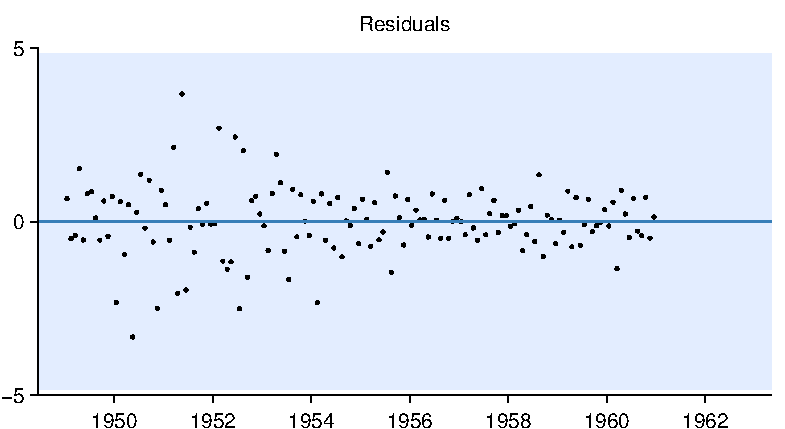
\includegraphics[trim=0 0 0 1.1cm, clip, width=0.5\textwidth]{figures/01-airline-months_resid.pdf}
      };
    \end{scope}
  \end{scope}
\end{tikzpicture}
